\section{Computational cost}\label{sec:cost}

\subsection{Labels}\label{sec:cost:labels}

In two dimensions the comparison of \cref{sec:results2d} used \numCmSolves{} solves,
\numCmSolvesVal{} for the 256 validation instances and \numCmSolvesTrain{} for the 1,024
labelled training instances, four load cases each; the run of 16 July 2026 used the same
labelled instances and a further \numTwoSolvesRun{} solves for the coarsened validation sets
of \cref{sec:results2d:other}. In three dimensions the comparison consumed
\numThreeSolves{}:
\numThreeTrainSolves{} for the 1,024 labelled training instances, \numThreeFewSolves{} for
the 64 fine-mesh instances reserved for few-shot training and \numThreeEvalSolves{} for the in-band and fine-mesh
validation sets. The validation solves are needed to evaluate any method; the training
solves are the price of supervision, and the label-free transformer needed none of them.

\subsection{Training}\label{sec:cost:training}

Label-free training of the three-dimensional transformer took \numTimeThreeSeed{} h per
seed on one NVIDIA GeForce RTX 5090, for 204,800 steps; the supervised transformer costs
the same per step, plus its labels. Full self-attention over all nodes dominates this cost
and grows with the square of the number of nodes: one training step took
\numEtwoTransformerFineStep{} s on a fine-mesh instance of \numEtwoNodesFine{} nodes. In
two dimensions, with the later code (\cref{sec:methods:networks}), three label-free seeds
trained in parallel on one GPU of the same type took \numTimeTwoParallel{}.

To reduce the cost of attention we tested, under a separate pre-registration, a
token-bottleneck network that pools the nodes into $M=512$ or $M=1{,}024$ tokens seeded by
farthest-point sampling, applies attention to the tokens only, and decodes each node from
a smooth blend of its six nearest tokens; it was trained on the energy alone, with every
other setting as for the transformer (\cref{tab:e2,fig:e2}). It trained
\numTimeBottleneckSpeedup{} times faster per seed (\numTimeBottleneckSeedMin{} h against
\numTimeThreeSeed{} h), but it was less accurate: its in-band relative energy gap was
\numEtwoGapMin{} to \numEtwoGapMax{} times the transformer's and its zero-shot fine-mesh
displacement error \numEtwoFineMin{} to \numEtwoFineMax{} times. Both variants were
dropped under their pre-registered accuracy criterion (\cref{tab:criteria}).

% generated by scripts/make_cmame_material.py from the records; do not edit
\begin{table}[tbp]
\centering
\footnotesize
\setlength{\tabcolsep}{4pt}
\caption{Token bottleneck against the transformer with one token per node, both trained on the energy alone with the same corpus, split, seeds and schedule (3D).}
\label{tab:e2}
\resizebox{\ifdim\width>\textwidth\textwidth\else\width\fi}{!}{%
\begin{tabular}{lccccc}
\toprule
Network & \shortstack{In-band \\ displacement} & \shortstack{In-band relative \\ energy gap} & \shortstack{Fine displacement \\ (zero-shot)} & \shortstack{Step (ms), \\ 12,318 nodes} & \shortstack{Step (ms), \\ 41,367 nodes} \\
\midrule
Transformer & 0.0300 $\pm$ 0.0028 & 0.00912 $\pm$ 0.00228 & 0.258 $\pm$ 0.045 & 1,415 & 14,795 \\
Bottleneck, M = 512 & 0.106 $\pm$ 0.051 & 0.0348 $\pm$ 0.0226 & 0.463 $\pm$ 0.082 & 27.8 & 49.2 \\
Bottleneck, M = 1,024 & 0.0892 $\pm$ 0.0096 & 0.0258 $\pm$ 0.0051 & 0.574 $\pm$ 0.059 & 36.9 & 47.5 \\
\bottomrule
\end{tabular}}

\smallskip
\begin{minipage}{\linewidth}\footnotesize\raggedright
M = 512: accuracy criterion, in-band relative energy gap +280.9\% (resolution 287\%), fine displacement +79.1\% (resolution 42\%; triggered); speed criterion, fine-mesh step 0.049 s against the 2.0 s limit: not triggered. Outcome: dropped.\par
M = 1,024: accuracy criterion, in-band relative energy gap +183.3\% (resolution 70\%; triggered), fine displacement +122.0\% (resolution 33\%; triggered); speed criterion, fine-mesh step 0.047 s against the 2.0 s limit: not triggered. Outcome: dropped.\par
Seeds per network: 3; seed mean $\pm$ sample SD. In-band: the 256 validation instances ($l_c$ = 0.0579--0.0906; the benchmark instances at the two ends of this range have 12,318 and 3,774 nodes); fine: 256 instances at $l_c$ = 0.0374 (41,367 nodes in the benchmark), never trained on. Errors are relative displacement error and relative energy gap.\par
Step time: one label-free training step on one instance of the stated size, NVIDIA GeForce RTX 5090, TF32 on, from a dedicated benchmark (bottleneck: the median over three repetitions of the time of 110 steps minus that of 10 steps, divided by 100, which removes the set-up time; transformer: a single timed step, its set-up included, the mean of its two benchmark measurements, 1,408 / 1,422 ms and 14,793 / 14,798 ms).\par
Resolution: the pre-registered max(10\%, 2 $\times$ SE$_\mathrm{rel}$), where SE$_\mathrm{rel}$ = $(s_\mathrm{T}^2/3 + s_\mathrm{B}^2/3)^{1/2}$ divided by the transformer's seed mean, with $s_\mathrm{T}$ and $s_\mathrm{B}$ the sample standard deviations of the two networks over the three seeds.
\end{minipage}
\end{table}


\begin{figure}[tbp]
\centering
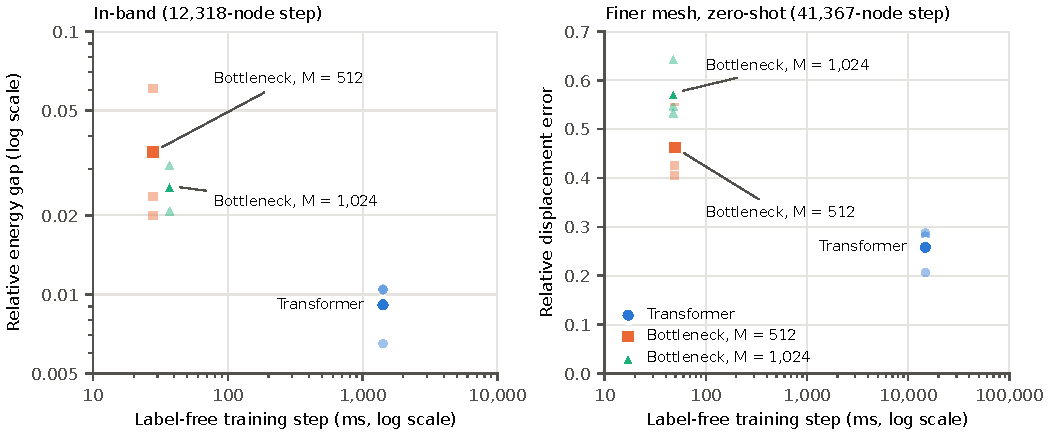
\includegraphics[width=\linewidth]{generated/fig_e2_cost_accuracy.pdf}
\caption{Cost against accuracy of the label-free transformer and the token bottleneck
(three dimensions, three seeds each; faint markers are seeds, ringed markers seed means).
Left: in-band relative energy gap against the time of one training step on an in-band
instance. Right: zero-shot fine-mesh displacement error against the time of one step on a
fine-mesh instance.}
\label{fig:e2}
\end{figure}

\subsection{Inference and solving}\label{sec:cost:inference}

\pending{A cost table: on the training machine and on the same validation and fine-mesh
instances, the time of surrogate inference (first call and repeated calls) against a
sparse direct solve, conjugate gradients from zero, conjugate gradients from the
prediction, and conjugate gradients stopped once the energy error of the iterate reaches
that of the prediction, with and without the rescaling of \cref{prop:amp}, together with
the surrogate's accuracy on those instances. The last two use the reference solution to
decide when to stop, so they give a lower bound on the time conjugate gradients need to
match the surrogate.}
